% Template for PLoS
% Version 1.0 January 2009
%
% To compile to pdf, run:
% latex plos.template
% bibtex plos.template
% latex plos.template
% latex plos.template
% dvipdf plos.template

\documentclass[10pt]{article}

% amsmath package, useful for mathematical formulas
\usepackage{amsmath}
% amssymb package, useful for mathematical symbols
\usepackage{amssymb}

% graphicx package, useful for including eps and pdf graphics
% include graphics with the command \includegraphics
\usepackage{graphicx}

% cite package, to clean up citations in the main text. Do not remove.
\usepackage{cite}

\usepackage{color} 

% Use doublespacing - comment out for single spacing
%\usepackage{setspace} 
%\doublespacing


% Text layout
\topmargin 0.0cm
\oddsidemargin 0.5cm
\evensidemargin 0.5cm
\textwidth 16cm 
\textheight 21cm

% Bold the 'Figure #' in the caption and separate it with a period
% Captions will be left justified
\usepackage[labelfont=bf,labelsep=period,justification=raggedright]{caption}

% Use the PLoS provided bibtex style
\bibliographystyle{plos2009}

% Remove brackets from numbering in List of References
\makeatletter
\renewcommand{\@biblabel}[1]{\quad#1.}
\makeatother


% Leave date blank
\date{}

\pagestyle{myheadings}
%% ** EDIT HERE **


%% ** EDIT HERE **
%% PLEASE INCLUDE ALL MACROS BELOW

%% END MACROS SECTION

\begin{document}

% Title must be 150 characters or less
\begin{flushleft}
{\Large
\textbf{I meant to do that: Extracting the intentions of action in the face of disturbances}
}
% Insert Author names, affiliations and corresponding author email.
\\
Justin Horowitz$^{1}$, 
James Patton$^{1,2\ast}$
\\
\bf{1} Bioengineering, University of Illinois at Chicago, Chicago, Illinois, United States
\\
\bf{2} Sensory Motor Performance Program, Rehabilitation Institute of Chicago, Chicago, Illinois, United States
\\
$\ast$ E-mail: pattonj@uic.edu
\end{flushleft}

% Please keep the abstract between 250 and 300 words
\section*{Abstract}
We derive a novel modeling approach for determining movement intent from a force-disturbed planar arm trajectory, examine its parameter sensitivity, and test the approach using human reaching data. We first show how to mathematically invert typical feedforward control approaches, and then examine how this reveals the strengths, limitations, and underlying assumptions. We found that sensitivity to parameter inaccuracies was on the order of microns and hence much lower than the inaccuracies seen when humans reach to visual targets. Further, most of the sensitivity resulted from uncertainty with regard to the joint stiffness. We also tested the robustness of this approach on human point-to-point reaching movements disturbed by force pulses. As expected, the intended trajectory showed no change from undisturbed reaching for 300 ms after the disturbance onset. Beyond this point, we detected change in intent even when the intention was near the target.  Unlike well-known $\lambda$ models, this intent was determined by considering both feedforward (predictive) and feedback controls. Knowing intent alongside action allows real-time determination and manipulation of error, even without a specified task, which makes it possible to directly inspect a neurally-impaired patient's intent for deficits. This approach may also be scaled for determining intent during human-machine interaction and in complex systems like team sports, crowds, or swarms.

% Please keep the Author Summary between 150 and 200 words
% Use first person. PLoS ONE authors please skip this step. 
% Author Summary not valid for PLoS ONE submissions.   
\section*{Author Summary}
In our everyday struggles with bumpy roads and bustling crowds we often make movements that do not match what we had planned. Here we identify a computational modeling method that measures actions and allows us to determine what the person meant to to do. We first demonstrate this method's good performance even when there is uncertainty in the parameters of the model. Next, we evaluate this on human reaching motions to targets, and show that while the arm is bumped by a disturbance, the intention remains straight. Approximately 300 milliseconds later, the intention changes in a corrective action that counteracts the disturbance. This type of computation can be broadly useful in canceling the effects of disturbances such as turbulence while typing or piloting, and can estimate intent in many other dynamic systems from molecules to crowds of people. It is also a new tool for understanding and treating impaired movement plans in neural injury.

\section*{Introduction}
There are many situations, such as disturbances, distractions, and pathologies, that interfere with execution of an intended movement. One can assume that a person who is familiar with a particular task will try to do the same thing each time, provided all other conditions are equal. This presumes that what people do is on average what they intended to do and that their goal remains unchanged. However, if there is a disturbance, it is unclear what happens to a person's intentions because action is decoupled from intention. Challenges arise in human-machine interactions because intention and changes in intention cannot be easily discerned. Hence a comprehensive method for understanding what someone means to do (rather than what they actually do or claim to have wanted to do) as they interact within uncertain environments will prove useful in any area where a person might be thwarted from their intent such as national security, operation of machinery, athletic and music performance, rehabilitation, human augmentation, and artificial intelligence.

It is important to distinguish our use of the term intent from other groups that consider \textit{motivation}\cite{mcclelland1985motives, rawolle2013relationships}, \textit{cost}\cite{todorov2002optimal, flash1985coordination}, or \textit{goal selection decisions}\cite{ziebart2010modeling}. In typical motor control studies, subjects are motivated to complete the experiment in a timely fashion and are usually explicitly provided targets to be reached. Classification of intent is prevalent in both lower \cite{strausser2011development, hargrove2013robotic} and upper limb\cite{englehart2003robust, young2012improving} prosthetics where hybrid control algorithms select from among a set of actions (walking/standing/flexion/extension/etc). While subjects may be \textit{motivated} to complete experiments with minimal effort/cost and their \textit{goal} may be to reach a target, here we use intent to describe the course of action (i.e., the trajectory of the arm) taken in service of goals and motives and not the goals nor the motives themselves. Particularly of interest is the intended course of action, even when the actual movement is disturbed and hence no longer matches the intent.

Attempts to deduce motor intent in the past have focused on the assumed spring-like properties of human muscles. Springs produce a force according to their impedance and stretch. By measuring force, impedance, and position, Gomi and Kawato\cite{gomi1997human} were able to deduce stretch and thereby infer the muscle's equilibrium point. Supporters of the "$\lambda$ model"\cite{feldman1995origin} hypothesized that this equilibrium point represented the intent of a movement. Upon Gomi and Kawato's inspection of the equilibrium point as it evolved in time, it was clear that it was highly complex and often not anatomically realizable. Therefore, it could not well-represent the intent of a simple reaching movement. We propose a revised method---intent extraction---that deduces intended trajectory, even in the face of disturbances. This method describes a class of filters that map a disturbance, process, actuator, and realized trajectory to an intended trajectory. In human reaching, the process (a dynamic model of the arm), the actuator (viscoelastic muscles), and the realized trajectory are all readily accessible via measurement and modeling. The mathematics underlying intent determination are sufficiently general to be extensible to whole-body movement or even more abstract, psychological processes.

Here we develop and analyze a method to extract intent from disturbed movement. This method then allows us to observe if and how intent changes following disturbance. We employ bidirectional modeling: we convert intent into movement using a forward model so that we can examine the quality and uncertainty of converting movement to intent by intent extraction. We then explore sensitivity and failure modes using standard model analysis techniques. We also demonstrate the accuracy and utility of this on a preliminary dataset of healthy reaching movements disrupted by occasional, unpredictable disturbances. We hypothesize that this combination allows intent extraction with less uncertainty than the uncertainty naturally inherent in point-to-point reaching. We show that certain factors and measurements are more sensitive than others, and demonstrate the viability of this method for providing a better understanding of what a person means to do when they move and are disturbed.


% You may title this section "Methods" or "Models". 
% "Models" is not a valid title for PLoS ONE authors. However, PLoS ONE
% authors may use "Analysis" 
\section*{Methods}
The sections below describe the theoretical method and the means by which we evaluate it. First, we considered an idealized system using synthetic data that demonstrated the concept and provided an understanding of the computational process. Next we conducted an experiment on humans to evaluate the process using human subject data. 

\subsection*{Intent Extraction: Deducing the Desired Trajectory}
We first demonstrate the \textit{intent extraction} approach in human motor control, but we later show that the process is applicable to any controlled process with an invertible highest order plant term. The process begins by presuming a model of the controller. Here, we choose the well-known motion control structure of Shadmehr and Mussa-Ivaldi\cite{shadmehr1994adaptive} where the feedforward aspect of the controller perfectly predicts the plant and linearizes the system through cancellation. Additionally, linear feedback rejects position and velocity error. This model was chosen to help illuminate the approach, but its feedback component lacks the complexity and accuracy of more recent approaches. Nevertheless later we will discuss how this approach can be used on more complex models without loss of generality. The equation governing the passive planar dynamics (plant) of musculoskeletal structure is of the form:
\begin{equation}
\underbrace{\overbrace{M(q)\ddot{q}}^{\text{Inertia}}+\overbrace{G(q,\dot{q})}^{\text{Coriolis, Centripal}}}_{\text{Plant}}+E=0
\end{equation}
Where $M$ is the mass matrix, $q$ is the joint angles, $\dot{q}$ is joint angular velocity, $\ddot{q}$ is joint angular acceleration, $G$ contains both Coriolis and centripetal effects, and $E$ is any externally-applied torque. The motion behavior changes with the addition of feedforward and/or feedback controllers:
\begin{equation}
\underbrace{\overbrace{M(q)\ddot{q}}^{\text{Inertia}}+\overbrace{G(q,\dot{q})}^{\text{Coriolis, Centripal}}}_{\text{Plant}}+E=\underbrace{\overbrace{\hat{M}(q_d)\ddot{q}_d}^{\text{Inertia}}+\overbrace{\hat{G}(q_d,\dot{q}_d)}^{\text{Coriolis, Centripal}}+\hat{E}}_{\text{Feedforward Controller}}+\underbrace{K_p(q_d-q)+K_d(\dot{q}_d-\dot{q})}_{\text{Impendance, Feedback Controller}}
\end{equation}
Some terms have hats over them ($\hat{M}$, $\hat{G}$, or $\hat{E}$) to indicate that they represent the nervous system's best estimate of the forces and dynamics it will encounter, which is also known as an internal model \cite{kawato1999internal}. This portion of the system serves as an inverse-dynamics feedforward controller that cancels out the dynamics of the arm in the torque balance. If the nervous system has sufficient experience and is expecting $E$, it is included as part of the internal model, $\hat{E}$, otherwise $\hat{E}$ is set to zero. $K_p$ and $K_d$ are the lumped impedance and feedback terms that employ a moving state equilibrium to accomplish the desired trajectory, $q_d$. This $q_d$ signifies the unknown desired trajectory that we seek to discover.

For typical dynamic simulations, in order to determine the trajectory of the system (i.e., the forward dynamics problem), this second-order differential equation is typically solved by numerical integration to determine the solution to the initial value problem in time. This first involves algebraic manipulation to solve for $\ddot{q}$, and then integration to determine the state trajectory. Intent determination takes the novel approach of instead solving for $\ddot{q}_d$:
\begin{equation}
\ddot{q}_d=\hat{M}(q_d)^{-1}\left\{M(q)\ddot{q}+G(q,\dot{q})+E-[\hat{G}(q_d,\dot{q}_d)+\hat{E}+K_p(q_d-q)+K_d(\dot{q}_d-\dot{q})]\right\}
\end{equation}  
$\ddot{q}_d$ can then be integrated to determine the intended state trajectory $q_d(t)$. This relies on many assumptions: The model of plant and controller must be accurate and precise. The initial conditions must be available and accurate. The mass matrix estimate, $\hat{M}$, must be invertible. Externally-applied force must be precisely and accurately measured. If all of these conditions are met, then the system yields an accurate estimate of the intent.

It is important to distinguish our intended trajectory, $q_d$, from another variable often considered, the equilibrium point of the muscle actuators. Importantly, this has been claimed to be the intended movement. To consider this, we also generalize our approach to any system with a moving intention that governs the control law. This introduces two additional layers of complexity by separating the plant (arm) into its process (dynamics) and actuator components (muscles) and considering the actuator's equilibrium, $q_e$ (sometimes represented as $\lambda$). The feedforward component must use and share this actuator and hence use the actuator's equilibrium. Without loss of generality, we represent the process $P$ and actuator $A$ as linear (or linearizable) operations in some space, $x$:
\begin{equation} \label{eq:generalPlant}
\underbrace{\overbrace{\sum_{n=1}^N P_nx^{(n)}}^\text{Process}+\overbrace{\sum_{m=1}^M A_m(x-x_e)^{(m)}}^\text{Actuator}}_\text{Plant}+E=0
\end{equation}
The internal model of the process ($\hat{P}$ and $\hat{E}$) predicts system actions, external disturbances, and impedance responses in order to determine $x_e$ that $x$ will track a desired path $x_d$.    
\begin{equation}
\overbrace{\sum_{n=1}^N \hat{P}_n x^{(n)}_d+\hat{E}}^\text{Internal Model}+\overbrace{\sum_{m=1}^M A_m(x_d-x_e)^{(m)}}^\text{Actuator}=0
\end{equation}
We solve this for $x_e$ and substituting into \eqref{eq:generalPlant} gives:
\begin{equation}
\overbrace{\sum_{n=1}^N P_nx^{(n)}}^\text{Process}+E=\overbrace{\sum_{n=1}^N \hat{P}_n x^{(n)}_d+\hat{E}}^\text{Internal Model}+\overbrace{\sum_{m=1}^M A_m (x_d-x)^{(m)}}^\text{Feedback (Actuator)}
\end{equation}

Note $x_e$ vanishes, recovering our familiar model. While a proper choice of $x_e$ is perhaps essential for control, our approach does not require a model relating equilibrium and intended trajectory. Note also that the actuator's equilibrium $x_e$ is not the process's equilibrium unless all derivatives of $x_d$ are zero. This upholds Gomi and Kawato's finding that the arm muscles' equilibrium does not represent reaching intent\cite{gomi1997human}. In summary, if the highest order coefficient of the dynamic model of the process $\hat{P}_N$ can be inverted and the impedances can be modeled, it is possible to solve for $x_d^{(N)}$ and integrate for $x_d$ revealing the intended trajectory.

While we treat both the process and actuator as dynamic models in our derivation, it is important to note that both the derivation and the technique are agnostic to the process model. Instead of a dynamic model, it could be a lookup table. For instance, a light switch is well-modeled as a lookup table or threshold without any consideration of its underlying mechanism. In this case, our technique could be used to determine a person's intention to flip the switch and how it changes in the face of disturbance. As long as some bidirectional relationship (even statistical) exists between state and outcome, intended outcome can be determined. This allows determination of intention in many situations of interest, even where the process is irreducibly complex.

\subsection*{Generation of synthetic data using simple dynamic simulation}
While the derivation above is general, testing its application to human reaching requires choices for plant and actuator models. Appropriate plant modeling is well-understand: measured arm segment lengths and self-reported body mass are converted into the plant's inertial, centripetal, and Coriolis terms. Anatomical landmarks and values from Dempster \cite{dempster1955space} and Winter \cite{winter2009biomechanics} relate body mass to limb mass, limb length to limb center of mass, and limb mass and length to moment of inertia. For the actuator, we choose the model of Burdet et al. \cite{burdet2006stability}. A scalar multiple of their modeled feedback torque, determined by linear regression, was used to account for any task-dependent differences in impedance \cite{franklin2003adaptation} while leaving the shape and structure of the impedance unchanged. As a consequence of choosing this model, muscle torque must be used to calculate stiffness even though it arises in part from stiffness. Like Burdet et al. \cite{burdet2006stability}, we approximated muscle torque by looking backward in time a small amount (500 microseconds). This approximation is not necessary during intent extraction, which leads to a small (sub-micrometer mean unsigned error) discrepancy. Desired trajectory in time was simulated as a minimum jerk, 5th order polynomial of duration 700 milliseconds starting and ending with zero velocity and acceleration.

\subsection*{Experimental Design}
Simulated reaches were 15 centimeters long, beginning 38 centimeters out from and 5.7 centimeters left of the right shoulder then proceeding right.  We used the following types of perturbing forces for each combination of distance and direction: 
pulse forces applied in one of the the two directions perpendicular to the direction of movement began when the subject had moved either 10\% or 50\% of the distance to the target and lasted for 150ms.
Noise forces began once the subject moved 3 millimeters, and lasted for the duration of the motion. The forces were drawn from a white noise generator at 1000 Hz with flat power spectral density of 1N, and then passed through a 4th order low-pass Butterworth filter with cutoff $10\pi$ rad/s. 

\subsection*{Error Metric}
Our error metric used deviation in position, where unsigned error was calculated as the mean magnitude of deviation from the nominal trajectory across each of 150 bins measuring 1 millimeter in width and spaced evenly throughout the 15 centimeter reach.  Mean unsigned error (MUE) was also used to summarize the overall error in each movement for sensitivity analysis. Mean and maximum signed error relative to the direction of disturbance, also called perpendicular deviation, were used to measure reaching accuracy in order to elucidate direction of any corrections.

\subsection*{Indices of variance-based sensitivity}
Sobol-distributed matrices were generated using MATLAB's sobolset() function and converted to parameter distributions (see Table~\ref{tab:parameters}) using inverse cumulative probability density. Distributions were clamped to the range of $\pm3$ standard deviations in order to limit parameters to a realistic range. Combinations and calculations were made as prescribed by Saltelli et al. \cite{saltelli2010variance} to arrive at direct and total sensitivity indices.

\subsection*{Human Subjects}
The human data trajectories analyzed here are drawn from four subjects who gave informed consent in accordance with Northwestern University Institutional Review Board, which specifically approved this study and follows the principles expressed in the Declaration of Helsinki. Two male and two female right-handed subjects (ages 24 to 30) performed the reaches with their right arm and were not compensated. Subjects' arm segment lengths were directly measured \textit{in situ} while body mass was self-reported.

\subsection*{Apparatus}
A planar manipulandum (described in Patton and Mussa-Ivaldi \cite{patton2004robot}) was programmed to compensate and minimize any friction or mass. The MATLAB XPC-TARGET package \cite{MATLAB:2008} was used to render this force environment at 1000 Hz and data were collected at 1000 Hz.  Visual feedback was performed at 60 Hz using OpenGL. Closed-loop data transmission time (position measurement to completed rendering to recognition of rendering by the position measurement system) was less than 8 milliseconds, ensuring a visual delay less than one 60 Hz frame.

\subsection*{Protocol}
Subjects made 730 reaches in total, along a line parallel to their coronal plane and approximately 45 centimeters from their shoulder. Reaches were either 15 or 30 centimeters long, starting and ending at one of three points spaced 15 centimeters apart on the line. To prevent any learning effect, forces were presented intermittently with random frequency, but never less than 5 reaches apart. Forces were chosen pseudorandomly such that each type, direction, and distance combination mentioned above was presented 5 times.  

\subsection*{Statistical Analysis}
The MATLAB statistics toolbox package \cite{MATLAB:2008} was used to perform comparisons among subjects and trajectory sources using ANOVA with Tukey-Kramer post-\textit{hoc} test for group differences.

% Results and Discussion can be combined.
\section*{Results}

\subsection*{Model Robustness}
While some inversion processes might be highly sensitive to model uncertainty, our process for recovering intent from action is much more precise than its input. Sensitivity analysis revealed that variance in intended trajectories due to estimated uncertainty in model parameters is lower than the natural variation in undisturbed motions.  Simulated point-to-point reaches disturbed by either filtered white noise forces or a pulse force perpendicular to the direction of the reach (Figure 1) were extracted in the presence of 220,000 variations upon the parameters (Table 1) according to the methods of Saltelli et al. \cite{saltelli2010variance}. Expected variance due to parameter uncertainty was $0.86  \mu m^2$ for pulse forces and $1.5 \mu m^2$ for filtered white forces. Variance in recorded undisturbed point-to-point reaching under the same time and reach distance conditions was $2.93 \mu m^2$. These variances all fall beneath the instantaneous accuracy of the robot recording the motion (tenths of a millimeter).

\subsection*{Parameter Sensitivity}
Simulated error due to direct parameter uncertainty (Figure 2) reached the order of millimeters and revealed particular sensitivity to misestimation of stiffness and changes in shoulder position from trial to trial. Direct sensitivity, which reveals the proportion of error that could be removed by correcting inaccuracy of a parameter, was an order of magnitude lower than total sensitivity, which reveals how much error would remain if all other parameters were accurate,  and both implicated stiffness estimation inaccuracy as a primary cause of extraction uncertainty. Note that this sensitivity analysis does not provide information on whether models or parameter estimates are accurate, only how sensitive the model would be if they were inaccurate. 

\subsection*{Human Intent Trajectories}
Extraction of intent from human point-to-point reaching revealed straight-line movement that persisted for hundreds of milliseconds after the onset of disturbing forces (Figure 3). In both pulse timing conditions, the intended trajectory remained straight towards the target, supporting the approach.  When disturbances occurred early in reaching, intent showed some signs of correction mid-reach. When disturbances occurred late in reaching, intent continued onto the target but then corrected anyways (Figure 3 lower plots). We observed no significant change of intent during force disturbance until 300 milliseconds after the onset of disturbance. Intention showed some systematic deflection toward the direction of disturbance peaking around 150 milliseconds after the onset of force disturbance, but this effect did not leave the range of error found in undisturbed movement. While the hand returns within 600 milliseconds to undisturbed levels of error, intention appears to first over-correct and is altered for as much as one second (Figure 4 shaded areas). 

We argue that the approach here represents the first sound method for looking at intent following disturbance, so we have only the undisturbed intention for comparison. If intent can change following disturbance, it can only do so after some period of time due to delay in processing sensory information and producing new motor commands. This represents a way to falsify the method: our determined intent should not diverge from the undisturbed intent of similar motions within this window of delay. We test this in Figure 4.

Following disturbance, we compare deviation in the hand and intended paths against the maximum deviation of undisturbed movements in order to determine at what point in time changes in hand path or intent can no longer be explained by normal variation and inaccuracy. Subjects' force-disturbed hand paths could no longer be explained ($p=0.05$) by deviation in undisturbed movement beginning within at most 135 milliseconds after the onset of disturbance. By contrast, intent did not change significantly for at least 300 milliseconds after the onset of disturbance (Table 2). This passes the test described above. While there does appear to be some systematic failure of the intent model to completely reject the disturbance, this residual disturbance does not exceed the statistical threshold for significance. An overcorrection beginning at approximately 200 milliseconds appears to account for change in intention in all subjects.


\section*{Discussion}
We sought to test the suitability and robustness of an algorithm that determines a person's intent during reaching motion, even if there are disturbances. Sensitivity analysis on synthetic data revealed that the method was suitable in that errors in response to parameter variations were smaller than trial-to-trial variance observed in human reaching. Significant misestimation could occur if the stiffness was inaccurately modeled. We tested this on human reaching and found that in spite of the hand being distubed by forces, the intended movement remained on-course to the target, perhaps changing between 200 and 300 milliseconds. This represents a new and accurate method for viewing intent and how it changes when faced with a force disturbance.

While the derivation of intent determination required many steps, the outcome is a filter whose use is straight-forward. Many filters for converting assumed intent into simulated hand trajectories have been proposed and validated \cite{shadmehr1994adaptive, franklin2003adaptation, burdet2006stability}. Demonstrating the validity and plausibility of mathematically transforming those filters to instead covert measured hand trajectories to intent adds a novel method to the arsenal of analytical methods for exploring human motor control.

The proposed approach could explain the discovery by Bizzi et al. \cite{bizzi1984posture} of a ``virtual trajectory'' ($\alpha$) in deafferented monkeys that progressed smoothly from the initial to final positions and how that virtual trajectory is different from $\lambda$. By deriving the technique in a general form, we discovered that our $x_d$ should be equivalent to $\alpha$ and can be used to determine the muscle equilibrium of a $\lambda$ model. $x_d$ and $\lambda$ are only equivalent when $x_d$ is not changing.  Even if the muscle equilibrium jumped abruptly, this would be insufficient to move the intended trajectory abruptly due to the presence of a virtual mass. This provides a striking and falsifiable prediction: reaching intention cannot jump abruptly.

Our analysis suggests that intent is slow to change if it changes at all following disturbance. While this work examines the time of onset of change, statistical testing cannot be used to detect the absence of change in an individual movement. Still, Figure 3 shows reaches that are more compatible with intermittent control than with continuous optimal feedback control. In classic optimal control, the system is always updating the intent in response to errors \cite{todorov2002optimal}. Our results suggest a latent response consistent with sensory feedback latencies \cite{pruszynski2012optimal}. Interestingly, disturbances that come later in the movement (Figure 3, bottom panel) appeared to not dramatically affect some subjects' intent, suggesting that people may stubbornly ``stick to their guns'' when they know that the stiffness and damping characteristics will provide enough restoring torque to arrive at the target. Time of response may be dependent on the time of the disturbance in the movement. Alternatively, control might be intermittent \cite{gawthrop2011intermittent} with limited opportunities to change intent. It remains to be seen if and how change in intent might be triggered. 

Determination of intent may facilitate motor training and stroke recovery. Error augmentation, which presently relies on dictating the reaching intent, has demonstrated the capacity to increase and speed up learning in healthy patients \cite{patton2004robot} and following stroke \cite{patton2006evaluation}. Augmentation of difference from static, dictated intent could be replaced with scaling of the magnitude of the difference between the desired and realized trajectory. This makes error augmentation during undirected reaching and exploration possible, including both error reduction and error magnification. Partial error cancellation would allow learning to take place without harm to task goals. As demonstrated by the success of the challenge-point framework \cite{guadagnoli2004challenge}, dynamic variation of augmentation as task learning progresses can be beneficial. With this extraction, error can be measured and augmented in real-time even without an explicit task, potentially enabling wider utility and application. 

This novel determination of intended trajectories from force-disturbed movements allows hypothesis testing that was not previously possible. This approach can take \textbf{any} ``candidate model'' of the human arm and create a filter that estimates the intended trajectory. By using tests such as the comparison with undisturbed straight line reaching employed in this paper, one can evaluate which candidate produces the most plausible intended trajectory, supporting one model over another.  Instead of comparing two generative models to see which better approximates movement, it is now possible to perform element-by-element fitting. Direct access to the intended trajectory allows optimal feedback control models to better understand and fit hypothesized cost functions and their parameters. In addition, mid-movement replanning became falsifiable: we were able to show that intended trajectories from disturbed motions differ from those undisturbed motions and how they differed.

The process model does not need to be explicitly formulated. Dynamic models that strive to understand intent are wide ranging, and can include mathematical models that range in application from national security to athletic performance. The plant (such as the actions of a crowd in a crowded square or the motions of an opposing team) may be too complex to model with simple linear transformations as we present above. However, by substituting some approximation or lookup table of input-outcome pairs, it is possible in a variety of applications to obtain the intent, even when disturbed. In other words, it may not be necessary to allow a bomber to succeed or an opposing team to be victorious to understand the plan behind their action.

Nevertheless, there are some limitations to these methods. Accurate interface force measurement (within a few tenths of a newton) is needed. Such instrumentation is available, but must be used with great care in order to preserve the accuracy of the estimate. Our sensitivity analysis on synthetic data revealed that slight error can lead to a trajectory that accumulates a drift due to bias caused by the force term. More importantly, while modern force sensors can be highly accurate with very high signal to noise ratios, they tend to drift over time, leading to error that can grow if the device is not periodically tared. Our empirical approach used several methods to mitigate these effects, and hence the errors became small. It remains to be seen if there are methods to further reduce the misestimation due to force error or eliminate the need for force estimation altogether.  

Our sensitivity analysis showed that approximation of stiffness is the most critical factor to accuracy in estimating intent. While serious trial-to-trial stiffness misestimation is unlikely, co-contraction in response to disturbance might plausibly double stiffness mid-reach. Even as the model is insensitive to normal variations, a human can halve or double their stiffness \cite{franklin2007endpoint} significantly reducing determination accuracy. These limitations are readily overcome by performing this sensitivity analysis on each force environment of interest and taking measures to detect co-contraction and hence stiffness alterations. Additionally, real-time determination of intent may allow real-time determination of stiffness.

Our simple linear scaling of Burdet et al.'s stiffness model \cite{burdet2006stability} facilitated hypothesis testing, but was inherently limiting. More accurate approaches would provide us with many free parameters through which to determine the outcome of the eventual extraction and obtain a spurious favorable result. Our results point to the possibility of the impedance changing during motion, perhaps as a function of time. As mentioned above, while this may be perceived as a shortcoming, it was necessary and can potentially be overcome in future work.

The general intent extraction approach presented here reveals the conditions needed to solve for the moving intent in an arbitrary dynamic process. Sensitivity analysis for this approach applied to the human arm demonstrated favorable conditions for determination of intent during force-disturbed reaching. Reaching intent became significantly different from baseline reaching only after enough time had elapsed for the disturbance to be processed and descending motor commands to change. This window into intent should allow advances in arm modeling, motor training, and human-machine interaction.

% Do NOT remove this, even if you are not including acknowledgments
\section*{Acknowledgments}
Research supported by NIH NS053606.  We thank Felix Huang, Jagan Jimmy, Christine Massie, Tejas Madhavan, and Mohi Ahmed for their review of preliminary manuscript. We also thank the community  of the Robotics Lab at the Rehabilitation Institute of Chicago for critical commentary during the genesis of this paper and the work leading up to it.
 
%\section*{References}
% The bibtex filename
\bibliography{paper1}

\section*{Figure Legends}
%\begin{figure}[!ht]
%\begin{center}
%%\includegraphics[width=4in]{figure_name.2.eps}
%\end{center}
%\caption{
%{\bf Bold the first sentence.}  Rest of figure 2  caption.  Caption 
%should be left justified, as specified by the options to the caption 
%package.
%}
%\label{Figure_label}
%\end{figure}

\begin{figure}[!ht]
\begin{center}
%\includegraphics[width=4in]{fig1.eps}
\end{center}
\caption{
{\bf Simulated data illustrating tautology of extraction absent parameter error across pulse and filtered Gaussian noise disturbance types.} Intent is modeled as a minimum jerk, 5th order polynomial. Forces experienced are combined with intent via Burdet et al.'s \cite{burdet2006stability} model to produce the simulated arm trajectory. Extraction to recover intention from arm and force trajectory follows.
}
\label{fig:synthetic}
\end{figure}

\begin{figure}[!ht]
\begin{center}
%\includegraphics[width=4in]{fig2.eps}
\end{center}
\caption{
{\bf Model sensitivity testing (from the variance-based method of Saltelli et al.\cite{saltelli2010variance}) reveals that the model is mostly sensitive to stiffness.} Parameter values are varied in a Sobol-distributed fashion according to Table 1. First order sensitivity, in purple, is the error that would be removed if the parameter was fixed at its nominal value. Total sensitivity, in teal, shows error that would remain if all other parameters were fixed at their nominal values.
}
\label{fig:sensitivity}
\end{figure}

\begin{figure}[!ht]
\begin{center}
%\includegraphics[width=4in]{fig3.eps}
\end{center}
\caption{
{\bf Subjects' disturbed hand trajectories and extraction of intended trajectories from them reveal that both variance and invariance of the motor plan can occur even in response to very large disturbances.} The hand path, in black, deviates from the green baseline, as a force pulse, gray arrows, are applied. This subject's extracted desired trajectories, in red (baseline in faded red), do not significantly differ from baseline during force application, but show some reaction afterwards.
}
\label{fig:anecdotes}
\end{figure}

\begin{figure}[!ht]
\begin{center}
%\includegraphics[width=4in]{fig4.eps}
\end{center}
\caption{
{\bf Comparison of subjects' perpendicular deviations across disturbed and undisturbed conditions reveals that intention is statistically indistinguishable from undisturbed reaching for at least 300 ms.} At most 135 milliseconds after the onset of disturbance, hand deviation in the presence of disturbance (black dots, black band is mean $\pm$ half of the critical value for simultaneous comparisons at 95\% confidence interval) can no longer be explained by undisturbed hand deviation (green band is mean maximum deviation). Movement intention (red dots, band is mean deviation) does not significantly deviate until at least 300 ms after the onset of disturbance.
}
\label{fig:grouptrends}
\end{figure}

\section*{Tables}
%\begin{table}[!ht]
%\caption{
%\bf{Table title}}
%\begin{tabular}{|c|c|c|}
%table information
%\end{tabular}
%\begin{flushleft}Table caption
%\end{flushleft}
%\label{tab:label}
% \end{table}

\begin{table}[!ht]
\caption{
\bf{Arm Parameter Values and Sensitivities}}
\begin{tabular}{|c|c|c c|c c|}
\hline
Parameter Name &
Units &
Nominal &
SD &
$S$ &
$S_T$ \\ \hline
Upper Arm Length ($L_1$) &
m &
0.33 &
0.01 &
0 &
0.10 \\
Forearm Length ($L_2$) &
m &
0.34 &
0.01 &
0 &
0.03 \\
Upper Arm Center of Mass Ratio ($\frac{L_{m1}}{L_1}$) &
1 &
0.436 &
0.0695 &
0 &
0.02 \\
Forearm Center of Mass Ratio ($\frac{L_{m2}}{L_2}$) &
1 &
0.682 &
0.0431 &
0 &
0.02 \\
Gross Body Mass ($m_g$) &
kg &
79.36 &
3.1 &
0 &
0.02 \\
Upper Arm Mass Ratio ($\frac{m_1}{m_g}$) &
1 &
0.028 &
0.0029 &
0 &
0.01 \\
Forearm Mass Ratio ($\frac{m_2}{m_g}$) &
1 &
0.022 &
0.0025 &
0 &
0.06 \\
Upper Arm Radius of Gyration Ratio &
1 &
0.322 &
0.0161 &
0 &
0.01 \\
Forearm Radius of Gyration Ratio &
1 &
0.468 &
0.0234 &
0 &
0.01 \\
Shoulder Parallel Coordinate &
m &
-0.057 &
0.02 &
0.02 &
0.18 \\
Shoulder Perpendicular Coordinate &
m &
0.88 &
0.02 &
0 &
0.08 \\
Force Sensor Miscalibration $x\text{-axis}$ &
N &
0 &
0.231 &
0 &
0.08 \\
Force Sensor Miscalibration $y\text{-axis}$ &
N &
0 &
0.1067 &
0.03 &
0.08 \\
Force Sensor Gaussian Noise SD $x\text{-axis}$ &
N &
0 &
0.1653 &
0 &
0.01 \\
Force Sensor Gaussian Noise SD $y\text{-axis}$ &
N &
0 &
0.2869 &
0 &
0.01 \\
Torque-Invariant Impedance Misestimation Ratio &
1 &
1 &
0.15 &
0.06 &
0.31 \\
Torque-Varying Impedance Misestimation Ratio &
1 &
1 &
0.15 &
0 &
0.15 \\
Damping-to-Stiffness Ratio ($k_d$) &
$\text{sec}^{-1}$ &
0.0833 &
0.0125 &
0 &
0.08 \\
Reflex Impedance Scale Factor &
1 &
0.02 &
0.003 &
0 &
0.04 \\
Reflex Damping to Stiffness Ratio ($g_d$) &
$\text{sec}^{-1}$ &
2 &
0.3 &
0 &
0.04 \\ \hline
\end{tabular}
\begin{flushleft}Synthetic model parameters and their associated mean (nominal) values and standard deviations (SD) used to determine the sensitivity indices of Saltelli et al. \cite{saltelli2010variance}. Also shown are the resulting sensitivity indices. Sensitivity indices less than one-thousandth were reported as zero. Total variance was $1.3 \mu m^2$, showing very small average deviations when using this approach. First-order sensitivity, $S$, can be interpreted as fraction of variance removable by perfectly correcting a factor. Total sensitivity, $S_T$, can be interpreted as the fraction left after correcting all other factors.
\end{flushleft}
\label{tab:parameters}
\end{table}

\begin{table}[!ht]
\caption{
\bf{Time Elapsed until Error in Undisturbed and Disturbed Reaching are Significantly Different}}
\begin{tabular}{|c|c|c|}
\hline
Subject Number &
Hand Deviation (milliseconds) &
Intent Deviation (milliseconds) \\ \hline
1 &
105 &
305 \\
2 &
105 &
405 \\
3 &
135 &
350 \\
4 &
105 &
300 \\ \hline
\end{tabular}
\begin{flushleft} ANOVA with Tukey-Kramer post-\textit{hoc} test ($p=0.05$) was used to simultaneously compare undisturbed hand maximum deviations to force-disturbed hand and intent deviations at 5 millisecond intervals. When  a significant difference was first detected, this was noted as the onset of deviation.
\end{flushleft}
\label{tab:onsets}
\end{table}

\end{document}